\documentclass[11pt,letterpaper]{article}
\usepackage[T1]{fontenc}
\usepackage{lmodern}
\ifdefined\pdfgentounicode
  \input{glyphtounicode}
  \pdfgentounicode=1
\fi
\usepackage[margin=1.1in]{geometry}
\usepackage{amsmath,amssymb,amsthm}
\usepackage{microtype,booktabs,tabularx,tikz,needspace}
\usepackage{hyperref}
\definecolor{linkblue}{RGB}{25,65,100}
\hypersetup{colorlinks=true,linkcolor=linkblue,citecolor=linkblue,urlcolor=linkblue,
  pdftitle={Computing Euclidean tensor prices},
  pdfsubject={Mean width, counting linear extensions, and the complexity of evaluation}}
\newtheorem{theorem}{Theorem}[section]
\newtheorem{proposition}[theorem]{Proposition}
\newtheorem{lemma}[theorem]{Lemma}
\newtheorem{corollary}[theorem]{Corollary}
\theoremstyle{definition}
\newtheorem{example}[theorem]{Example}
\newcommand{\E}{\mathbb E}
\newcommand{\R}{\mathbb R}
\newcommand{\Q}{\mathbb Q}
\newcommand{\C}{\mathbb C}
\newcommand{\Prob}{\mathbb P}
\newcommand{\sharpP}{\#\mathrm P}
\newcommand{\PSPACE}{\mathrm{PSPACE}}
\newcommand{\etr}{\exists\R}
\newcommand{\norm}[1]{\lVert#1\rVert}
\newcommand{\ip}[2]{\langle #1,#2\rangle}
\newcommand{\wire}{\mathsf W}
\DeclareMathOperator{\rank}{rank}
\DeclareMathOperator{\Var}{Var}
\title{The complexity of computing Euclidean tensor prices}
\author{}
\AddToHook{cmd/maketitle/after}{%
  \par\noindent\begin{minipage}{\linewidth}
  \small\sffamily
  I asked ChatGPT these questions to understand what follows from the recent
  VP versus VNP breakthrough. I share its answers so that these explorations
  are available beyond a private conversation. These are AI-generated notes,
  not research papers. I do not claim authorship or priority for the ideas.
  Arguments may be wrong, and earlier work may be overlooked or misattributed.
  I welcome corrections by mail or via
  \href{https://github.com/radomite/algebraic-complexity/issues}{GitHub}.
  \end{minipage}\par\medskip
}
\AddToHook{shipout/foreground}{%
  \ifnum\ReadonlyShipoutCounter>1\relax
  \put(0pt,-24pt){\makebox[\paperwidth][c]{%
    \normalfont\sffamily\fontsize{8}{10}\selectfont\color[gray]{0.38}%
    AI-generated exploration notes. Arguments and attributions may be wrong.
    \href{https://github.com/radomite/algebraic-complexity/issues}{Corrections welcome on GitHub.}}}%
  \fi
}

\begin{document}
\maketitle

\section{One bit at many sites}
\label{sec:intro}

Place the indices of \(e_0\otimes e_0+e_1\otimes e_1\) at points \(x,y\).
The tensor carries a single bit across the segment from \(x\) to \(y\), at a
price of \(\norm{x-y}\). Place a third copy of the same bit at \(z\).
If the three sites form a triangle, the price becomes half its perimeter.
At more sites the same rule has a Gaussian description. For a finite
nonempty \(S\subset\R^d\) and \(g\) a standard Gaussian vector, put
\begin{equation}
 W(S)=\sqrt{2\pi}\,\E\max_{v\in S}\ip{g}{v}.
 \label{eq:width}
\end{equation}
Translating all sites adds a centered Gaussian to the maximum, preserving
its expectation. After translation, only the projection of \(g\) onto the
span of the sites matters.
The Euclidean price theorem assigns the tensor
\(\Delta^{(k)}_2=e_0^{\otimes k}+e_1^{\otimes k}\) the price \(W(S)\)
when its \(k\) indices occupy precisely the sites in \(S\). This holds over
every coefficient field. Our first problem takes the two nonzero words
and the list of sites as input. All the computational difficulty can
therefore reside in the coordinates. \cite[Theorem~1.1]{euclid}

\begin{theorem}\label{thm:main}
Given \(k\) rational sites in binary and a precision parameter \(s\), computing
the price of \(\Delta^{(k)}_2\) within \(2^{-s}\) is polynomial-time
Turing-equivalent to a \(\sharpP\) oracle. Hardness holds with all sites of
norm at most \(\sqrt 2\). At integer sites of unrestricted magnitude even
additive error one is \(\sharpP\)-hard. In each fixed affine dimension
the \(2^{-s}\)-accuracy problem is in deterministic polynomial time.
In arbitrary dimension there is a fully polynomial randomized relative
approximation scheme.
\end{theorem}

\Needspace{5\baselineskip}
Here \(\sharpP\) consists of the functions counting binary witnesses of
polynomial length accepted by a polynomial-time predicate. A numerical
oracle may return any dyadic approximation on the \(2^{-s}\) grid within
the stated error. Our reduction works for every valid rounding. Conversely,
a deterministic machine with a counting oracle produces such an answer.
We measure time in the binary input length and \(s\), equivalently with
\(s\) in unary. All logarithms are to base two.

Table~\ref{tab:inputs} compares three encodings. An explicit dense input
lists every rational coefficient. Listed support gives the index and
coefficient of each nonzero entry. A succinct input here is a Boolean
circuit that returns a zero--one entry on binary indices.

\begin{table}[htbp]
\centering\small
\begin{tabularx}{\linewidth}{@{}p{.38\linewidth}X@{}}
\toprule
Input and sites & Evaluation or decision problem\\
\midrule
Shared bit, listed sites & High precision has the Turing degree of \(\sharpP\)
(\S\S\ref{sec:count}--\ref{sec:algorithms}).\\
Explicit tensor at \(0,\lambda,1\) & Numerical evaluation and exact equality
are in P for rational \(\lambda\). Exact ordering at the midpoint is equivalent
to unary square-root sum (\S\ref{sec:line}).\\
Independent wires, integer endpoints & Numerical evaluation is in P.
Exact ordering in growing dimension is equivalent to binary square-root sum
(\S\ref{sec:line}).\\
Circuit-specified matrix, unit segment & Full-rank price is \(\PSPACE\)-complete.
Additive error one is NP-hard even for diagonal matrices (\S\ref{sec:succinct}).\\
Unknown entries or sites & Minimizing an affine matrix price and realizing unit
wire prices in the plane are \(\etr\)-complete (\S\ref{sec:inverse}).\\
\bottomrule
\end{tabularx}
\caption{The precision parameter and the tensor representation are part of the problem.}
\label{tab:inputs}
\end{table}

\subsection*{What makes a value a price?}
For a field \(K\), a tensor \(T\in V_1\otimes\cdots\otimes V_k\) has one
finite-dimensional factor, or leg, at each listed position \(x_i\).
When several legs share a site, group their spaces by tensor product. Give
an unused site a one-dimensional space. A \emph{restriction} applies one
linear map at each site. A \emph{direct sum} \(T\oplus U\) puts the two
tensors in separate blocks at every site. The product \(T\boxtimes U\)
groups the corresponding legs of the ordinary tensor product.

On a fixed finite set \(S\) of positive diameter a \emph{spectral point}
\(F_S\) takes nonnegative real values, sends zero to zero and the unit
tensor to one, adds on direct sums, multiplies on products, and can only
decrease under restriction. The Euclidean theorem supplies such points
simultaneously on every finite set in a real Hilbert space. Their prices
\(H(T;x)=W(S)\log F_S(T)\) agree upon enlarging \(S\). For nonzero \(T\)
they depend only on the labeled distances and scale linearly when the
placement is dilated. A label shared among a set \(S\) has price
\begin{equation}
 H(\Delta_S(q))=W(S)\log q,\qquad
 \Delta_S(q)=\sum_{a=1}^q\bigotimes_{v\in S} e_a .
 \label{eq:diagonal}
\end{equation}
We call any system satisfying these properties \emph{compatible}. A
nonzero tensor at a single site costs zero. We use \(H(0)=-\infty\).
Any nonzero tensor restricts to the unit by selecting a nonzero coefficient,
so its price is nonnegative. Repeating a label at a site preserves its price
because \(e_a\) and \(e_a^{\otimes j}\) are interconvertible on their
spans by local linear maps. \cite[Theorem~1.1]{euclid}

The \(q\)-valued wire \(\wire_{ij}(q)\) is \(\Delta(q)\) on sites \(i,j\)
with unit factors elsewhere. Contracting one end against a leg of
dimension \(q\) transports that leg to the other end. The contraction sends
\(e_a\otimes e_b\) to \(\mathbf1_{a=b}\). Moving the legs in both directions gives
\begin{equation}
 |H(T;x)-H(T;y)|\le\sum_i(\log\dim V_i)\norm{x_i-y_i}\qquad(T\ne0).
 \label{eq:transport}
\end{equation}
Two-site tensors are matrices. Row and column operations identify a
rank-\(r\) matrix with a wire of dimension \(r\), up to unused dimensions.
At distance \(L\) its price is \(L\log r\). A product of independent wires
costs the sum of their individual prices. Rational Gaussian elimination
therefore prices an explicit matrix to any prescribed precision in
polynomial bit time, using a square root for \(L\) at rational sites.

\section{Counting linear extensions with two placements}
\label{sec:count}

Let \(P\) be a poset on the listed elements \(1,\ldots,n\), with \(m\)
generating relations \(i\prec j\). A \emph{linear extension} is a permutation
in which every \(i\) precedes its successors. Write \(e(P)\) for their number.
In \(\R^{n+1}\) use the standard basis and form
\[
 S_0=\{0\}\cup\{e_i-e_j:i\prec j\text{ is listed}\},\qquad
 S_h=S_0\cup\{h e_{n+1}\}.
\]
The same shared bit has \(m+2\) legs in both queries. One leg sits at the
origin, one at each listed difference, and the last moves from the origin
to \(he_{n+1}\). Write \(W_0=W(S_0)\) and \(W_h=W(S_h)\).
In the original \(n\) coordinates the origin maximizes the projection
exactly on the \emph{order cone} \(\{g:g_i\le g_j\text{ whenever }i\prec j\}\).
Its braid chambers correspond to linear extensions~\cite[Section~2.4]{dbkr-poset-cones}. Applying the standard normal distribution function coordinatewise turns this probability into the volume of Stanley's order polytope~\cite[Corollary~4.2]{stanley-poset-polytopes}. The extra coordinate measures the cone probability from width queries.

\begin{lemma}\label{lem:lift}
For every \(h>0\),
\[
 0\le \frac{W_h-W_0}{h}-\frac{e(P)}{n!}\le \frac{mh}{2\sqrt2}.
\]
\end{lemma}
\begin{proof}
Take independent standard normals \(g_1,\ldots,g_n,Z\) and put
\(M=\max(\{0\}\cup\{g_i-g_j:i\prec j\text{ is listed}\})\).
Writing \(a_+=\max(a,0)\), equation~\eqref{eq:width} gives
\[
 W_h-W_0=\sqrt{2\pi}\,\E(hZ-M)_+ .
\]
The \(g_i\) almost surely have a strict order, uniform among the \(n!\)
permutations. Exactly \(e(P)\) orders satisfy \(M=0\). On this event the
new point contributes \(hZ_+\), independently of the order, and
\(\sqrt{2\pi}\E Z_+=1\). Its contribution to the width is \(h e(P)/n!\).

If \(0<M<t\), some listed difference belongs to \((0,t)\).
Each difference has law \(N(0,2)\) with density bounded by
\(1/(2\sqrt\pi)\). A union bound gives
\(\Prob(0<M<t)\le mt/(2\sqrt\pi)\). For \(M>0\) the additional contribution
to the maximum lies between zero and
\(hZ_+\mathbf1_{\{0<M<hZ_+\}}\). Condition on \(Z\), apply the union
bound, and use \(\E Z_+^2=1/2\). The remainder in the width is at most
\(\sqrt{2\pi}\,mh^2/(4\sqrt\pi)=mh^2/(2\sqrt2)\).
\end{proof}

Choose
\[
 b=\lceil\log(8(m+2)n!)\rceil,\qquad h=2^{-b},\qquad s=2b .
\]
Each price can have error \(h^2\). After subtracting, dividing by \(h\),
and multiplying by \(n!\), the total error is at most
\((m+2)n!h\le1/8\). Rounding recovers the integer \(e(P)\). Both queries
are specified before either answer arrives, every site has norm at most
\(\sqrt2\), and \(b=O(n\log(n+1)+\log(m+2))\). Counting linear extensions
is \(\sharpP\)-complete under polynomial-time Turing reductions. This
proves the bounded-coordinate lower bound in Theorem~\ref{thm:main}.
Dilating both configurations by \(h^{-2}\) makes the coordinates integers
of polynomial bit length. An error of one then rescales to \(h^2\), proving
the unit-error assertion. \cite{brightwell-winkler-extensions}

\begin{figure}[htbp]
\centering
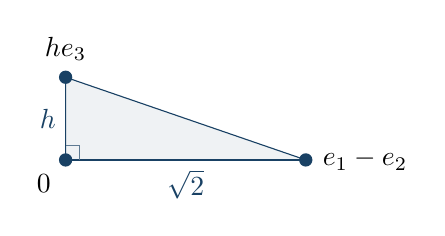
\begin{tikzpicture}[x=1cm,y=1cm,ball/.style={circle,fill=linkblue,inner sep=1.7pt}]
  \coordinate (o) at (0,0); \coordinate (a) at (3.05,0);
  \coordinate (z) at (0,1.05);
  \fill[linkblue!7] (o)--(a)--(z)--cycle;
  \draw[linkblue,thick] (o)--node[below] {\(\sqrt2\)} (a);
  \draw[linkblue] (o)--node[left] {\(h\)} (z)--(a);
  \draw[linkblue!70] (.18,0)--(.18,.18)--(0,.18);
  \node[ball,label=below left:\(0\)] at (o) {};
  \node[ball,label=right:\(e_1-e_2\)] at (a) {};
  \node[ball,label=above:\(he_3\)] at (z) {};
\end{tikzpicture}
\caption{One relation \(1\prec2\). Moving the duplicate leg off the base
segment produces a right triangle in its affine plane.}
\label{fig:one-relation}
\end{figure}

For a planar convex polygon and a direction \(g\), summing
\(\lvert\ip{g}{e}\rvert\) over its cyclic edge vectors gives twice its
projection range \(Y(g)\). Each of the two boundary chains covers the
projected interval once. By Gaussian symmetry \(W=\sqrt{\pi/2}\,\E Y\),
and \(\E|\ip{g}{e}|=\sqrt{2/\pi}\norm e\). Thus \(W\) is half the
perimeter, and a segment has width equal to its length. In
Figure~\ref{fig:one-relation} this gives the exact difference quotient
\[
 \frac{W_h-W_0}{h}
 =\frac12+\frac{h}{2(\sqrt{2+h^2}+\sqrt2)} .
\]
The first term is the probability of the order \(g_1<g_2\). The second
is the contribution from projections in which the new point overtakes a
positive old maximum.

\section{Algorithms for the shared bit}
\label{sec:algorithms}

\subsection{High precision with a counting oracle}
Translate one site to the origin. The maximum
\(f(x)=\max_{v\in S}\ip{v}{x}\) is now nonnegative and \(A\)-Lipschitz,
where \(A\ge1\) is an integer bounding every \(\norm v\). For example,
round up one plus the sum of the absolute input coordinates after translation.
The normalized Gaussian integral outside \([-R,R]^d\) is bounded by
\[
 \sqrt{2\pi}\,A\sqrt{\E\norm g^2\,\Prob(\norm g_\infty>R)}
 \ \le\ 2\sqrt\pi\,A d\,e^{-R^2/4}.
\]
Here Cauchy--Schwarz, \(\E\norm g^2=d\), and a union bound over the
Gaussian tails suffice. Take an integer \(R=O(1+s+\log(Ad))\) making this
bound smaller than \(2^{-s-3}\). The case \(d=0\) returns zero.

On the box, the integrand
\(u(x)=(2\pi)^{(1-d)/2}f(x)e^{-\norm x^2/2}\) has Lipschitz constant
at most \(A(1+dR^2)\). Indeed \(f(x)\le AR\sqrt d\), and the gradient of
the exponential there has norm at most \(R\sqrt d\). A corner sum on a
cubical grid of mesh \(2^{-k}\) therefore has error at most
\[
 (2R)^d A(1+dR^2)\sqrt d\,2^{-k}.
\]
Choose \(k\) to make this less than \(2^{-s-3}\). A cell address has only
\(O(d(k+\log(2R)))\) bits. At its lower corner \(y\), compute a
nonnegative integer \(w_y\) with
\[
 \big|2^{-q}w_y-u(y)\big|\le 2^{1-q},
 \qquad q=s+\lceil d\log(2R)\rceil+5 .
\]
The dot products are rational. Polynomial bit time suffices for the
remaining operations. Use the Taylor series with guard bits for the
exponential on a polynomially bounded interval, and the geometrically
convergent arctangent series at \(1/5,1/239\) in Machin's formula for
\(\pi\). Rational powers of the normalizing constant require only integer
powers and a square root. Rounding an approximation of \(u(y)\) to the
nearest nonnegative multiple of \(2^{-q}\) gives the asserted tolerance.

A counting machine guesses one cell address and one integer \(z\) in
fixed-length binary, and accepts exactly when the address is valid and
\(0\le z<w_y\). The bound \(u(y)\le AR\sqrt d\) supplies a polynomial
length for the second guess. The count is exactly \(\sum_y w_y\).
Multiplication by \(2^{-kd-q}\) converts this integer to a width estimate.
The weight errors contribute at most \((2R)^d 2^{1-q}\). Together with
the tail and grid errors this leaves room for final rounding to the
\(2^{-s}\) grid. This proves the upper reduction in Theorem~\ref{thm:main}.

\subsection{Deterministic integration in fixed affine dimension}
First suppose the sites lie in \(\Q^r\), with \(r\ge1\) fixed. Remove
duplicates and intersect the truncated box with the inequalities
\(\ip{x}{v-w}\ge0\) for every \(w\in S\), in turn for each \(v\in S\).
These rational polytopes cover the box. Their full-dimensional interiors
are disjoint, and on the cell for \(v\) the function \(f\) equals \(\ip{x}{v}\).

Enumerate vertices by solving \(r\) independent tight inequalities and
checking all constraints. Each nonempty face is obtained by imposing at most
\(r\) independent tight constraints and collecting the vertices on them.
Deduplicate the vertex lists and discard cells of dimension less than
\(r\). Cone each face boundary to the average of its vertices, starting
with edges. The resulting triangulation has one simplex for each maximal
chain of faces. In fixed dimension it has polynomially many simplices,
with rational coordinates of polynomial bit length.

For \(t=\norm{x}^2/2\le rR^2/2\), the Taylor polynomial for \(e^{-t}\)
of degree \(j-1\) has error at most \(t^j/j!\le(et/j)^j\). Take
\(j\ge erR^2\) large enough that \(2^{-j}(2R)^rAR\sqrt r<2^{-s-3}\).
Integrate the product of this polynomial and the linear function on each
simplex exactly. After an affine substitution with its absolute Jacobian,
the only integrals needed are
\[
 \int_{\{x_i\ge0,\ \sum_i x_i\le1\}} x^\alpha\,dx
   =\frac{\prod_i\alpha_i!}{(r+|\alpha|)!},
\]
by successive one-variable integrations. In fixed dimension both the number
of monomials and every rational bit length are polynomial in the input and
\(s\). Multiply by \((2\pi)^{(1-r)/2}\) to sufficient precision. The
tail estimate and the uniform Taylor error give the result.

For sites of affine dimension \(r\) in a larger space, translate first and
choose an independent rational basis of their span by elimination.
Orthogonalize over \(\Q\) before normalizing. Each coordinate of a site in
the resulting frame is a rational dot product divided by the square root
of a positive rational. Gram determinants bound their intermediate bit
lengths polynomially. Moving each site by at most \(\eta\) in \(\R^r\)
changes \(W\) by at most \(\sqrt{2\pi}\,\eta\,\E\norm g
\le\sqrt{2\pi r}\,\eta\). Dyadic coordinates computed with a few guard
bits therefore suffice. For \(r=0\) the answer is zero.

There is also a bound for the dense encoding of this particular tensor.
With \(k\) binary legs the input length \(N\) is at least \(2^k\), and
\(r\le k-1\). A cell has at most \(k+2r\) defining inequalities, at most
\(2^{k+2r}\) faces, and at most \(2^{O(k^2)}\) maximal face chains.
Its vertices have polynomial bit length, and a face average sums at most
\(2^{O(k)}\) such vertices. The Taylor degree is polynomial in \(N+s\),
so each substituted polynomial has at most \((N+s+2)^{O(k)}\) monomials.
Powers of coordinates multiply their bit lengths by at most the degree.
In addition one may use the product of all the summands' denominators as
a common denominator, whose bit length is at most their total bit length.
These estimates give a deterministic \((N+s+2)^{O(\log(N+s+2))}\) time
bound. The poset reduction uses the two-word description of the tensor.

\subsection{Relative error from random projections}
Let \(D\) be the diameter of the sites. If \(D=0\), return zero. For
\(D>0\) consider the projection range
\[
 Y(g)=\max_{v,w\in S}\ip{g}{v-w}.
\]
Symmetry gives \(W=\sqrt{\pi/2}\,\E Y\).
Meka~\cite[Introduction and Theorem~1.2]{meka-gaussian} discusses Gaussian sampling and gives a deterministic PTAS for expected Gaussian suprema. The symmetric set of differences \(S-S=\{v-w:v,w\in S\}\) gives the supremum above. We analyze a randomized implementation with rational input and explicit bit precision.

A diameter pair gives
\(\E Y\ge\sqrt{2/\pi}\,D\), while the maximum formula makes \(Y\)
\(D\)-Lipschitz. Maurey's Gaussian rotation argument, as presented by Pisier~\cite[Theorem~2.2]{pisier-gaussian}, gives a variance estimate independent of the ambient dimension.

\begin{lemma}
\(\Var Y(g)\le\pi^2D^2/8\).
\end{lemma}
\begin{proof}
For independent standard Gaussian vectors \(g,g'\), put
\(g_t=g\cos t+g'\sin t\) for \(0\le t\le\pi/2\).
At each fixed \(t\), \(g_t\) and its derivative \(\dot g_t\) are
independent standard Gaussian vectors, by orthogonal invariance.
The maximum of finitely many linear functions is differentiable off
a finite union of hyperplanes, with gradient of norm at most \(D\).
Integrating along the curve and applying Cauchy--Schwarz gives
\[
 2\Var Y=\E\big[(Y(g')-Y(g))^2\big]
 \le\frac{\pi}{2}\int_0^{\pi/2}
       \E\big[\ip{\nabla Y(g_t)}{\dot g_t}^2\big]\,dt
 \le\frac{\pi^2}{4}D^2 .
\]
The last expectation, conditional on \(g_t\), is the squared gradient norm.
\end{proof}

For \(0<\varepsilon,\delta<1\), average \(O(\varepsilon^{-2})\)
independent copies of \(Y\) in a group. Chebyshev's inequality bounds its
relative error by \(\varepsilon/2\) with probability at least \(3/4\)
for a suitable constant. A median of \(O(\log(2/\delta))\) independent
groups fails with probability at most \(\delta/2\), by the binomial tail
bound. Thus \(T=O(\varepsilon^{-2}\log(2/\delta))\) Gaussian vectors suffice.

For a bit implementation choose an integer \(R=O(1+\log(2dT/\delta))\)
so that all \(dT\) coordinates lie in \([-R,R]\) except with probability
\(\delta/4\). Clip and round each coordinate to a grid of step at most
\(\varepsilon/(32d)\). On this event the error in each range is at most
\(D\varepsilon/32\). The grid has polynomial size in \(d,1/\varepsilon\)
and \(\log(2/\delta)\). Approximate its one-dimensional cumulative bin
probabilities by integrating the Gaussian from zero to each boundary,
using symmetry, endpoint tails, and the Taylor bound above. Round the
cumulative values on a common dyadic grid, take prefix maxima to enforce
monotonicity, and set the last value to one. With \(J\) bins, accuracy
\(\delta/(16JdT)\) per cumulative value suffices for total variation at
most \(\delta/(4dT)\) per coordinate. A uniform binary integer samples
this dyadic law exactly. Coupling all coordinates costs at most another
\(\delta/4\) in failure probability. Computing \(\sqrt{\pi/2}\) within
relative error \(\varepsilon/16\) finishes the bit algorithm. Its running
time is polynomial in the input length, \(1/\varepsilon\) and
\(\log(2/\delta)\).

For a poset with at least one listed relation, \(W_0\ge\sqrt2\) because
the base contains a segment of that length. To guarantee additive error
\(h^2\) there by relative approximation requires
\(\varepsilon\le h^2/W_0\). Thus the sampling bound can be exponential
in the number of precision bits used in Lemma~\ref{lem:lift}.

\Needspace{12\baselineskip}
\section{Three sites on a line}
\label{sec:line}

Let an explicit rational tensor have its legs at \(A=0,B=\lambda,C=1\),
where \(0<\lambda=u/v<1\) is rational in binary. The interval has width
one. Its endpoint wire of dimension \(q\) attains the full spectral value
\(q\), even when the middle site is available. This identifies the price of
every tensor on the interval by a theorem about three-tensor spectral points.

\Needspace{9\baselineskip}
\begin{theorem}\label{thm:line}
At the sites \(0,\lambda,1\), the price of a nonzero explicit rational
three-tensor is forced. There are polynomial-time computable dimension
pairs \((a_j,c_j)\), independent of \(\lambda\), such that
\begin{equation}
 H(T)=\log\!\left(\sum_j a_j^\lambda c_j^{1-\lambda}\right).
 \label{eq:line}
\end{equation}
Numerical evaluation and exact equality of two prices take deterministic
polynomial time, including the binary length of the rational division.
This holds for dense and listed-support input. At the midpoint, exact
ordering is polynomial-time many-one equivalent to comparison of two sums
of square roots of unary integers.
\end{theorem}
\begin{proof}
The edge theorem of Alman, Li and Pratt says that a spectral point taking
the full dimension on the endpoint wire belongs to the family of
\emph{edge support functionals} with weights \((\theta_A,0,\theta_C)\),
\(\theta_A+\theta_C=1\). The value of an \(ij\) wire is \(q^{\theta_i+\theta_j}\).
Fix the middle index and regard the slices as maps from the dual of the
left space to the right space. A filtration is a nested chain of pairs of
source and target subspaces, with each slice mapping every source into
its paired target. The slope of a nonzero pair is the ratio of the source
and target dimensions, with value infinity when the target is zero.
The Harder--Narasimhan filtration has successive quotients of strictly
decreasing slopes, and no invariant subpair of a quotient has larger slope
than that quotient. The theorem gives the functional as
\(\sum_j a_j^{\theta_A}c_j^{\theta_C}\), where \((a_j,c_j)\) are the
successive quotient dimensions. They can be computed exactly in
deterministic polynomial bit time on rational input.
\cite[Theorems 1.2 and 1.6, Corollary 9.2 and Remark 9.3]{alp-edge}

The costs of the wires \(AB\) and \(BC\) force
\(\theta_A=\lambda\) and \(\theta_C=1-\lambda\), giving~\eqref{eq:line}.
Each positive dimension increment is bounded by its endpoint dimension.
The sum and its logarithm can be evaluated to \(s\) bits in polynomial
time by writing each power using a logarithm and an exponential. On a
nonzero tensor the sum is at least one. If \(t\) entries are listed,
restrict each local basis to its at most \(t\) active coordinates.
Zero padding reverses this restriction. The new dense input has at most
\(t^3\) coefficients. Zero tensors can be treated separately.

For equality, discard terms with a zero factor. Factor the remaining
dimensions by trial division, which is polynomial here because their
values are bounded by the explicit input size after compression. For
every prime \(p\) and pair \(a,c\) compute
\[
 u\nu_p(a)+(v-u)\nu_p(c)=v q_p+r_p,\qquad 0\le r_p<v .
\]
Its term is an integer coefficient \(\prod_p p^{q_p}\) times the radical
\(\prod_p p^{r_p/v}\). Distinct remainder vectors give radicals with
irrational ratio, since the valuations of a rational \(v\)-th power
are multiples of \(v\). A theorem of Carr and O'Sullivan says that real
\(v\)-th roots of rationals which are pairwise linearly independent over
\(\Q\) are jointly linearly independent. Thus two sums agree precisely
when their integer coefficients agree after collection by remainder
vector. Each coefficient before collection is at most \(\max(a,c)\),
and the integer divisions use polynomially many bits even for large \(v\).
For two different rational divisions of unit intervals, use the least common
multiple of the denominators. \cite[Theorem~1.1]{carr-osullivan-roots}

At \(\lambda=1/2\) the terms are \(\sqrt{a_jc_j}\) and their radicands
can be written in unary in polynomial time. In the reverse direction,
given positive integers \(b_j\) in unary, take the direct sum of the
\(\wire_{AB}(b_j)\), each with a one-dimensional factor at \(C\).
The direct sum uses a separate block at \emph{every} site, so its value
is exactly \(\sum_j\sqrt{b_j}\). Its dense array takes polynomial time to
write. The logarithm is increasing.
\end{proof}

For example, the two lists \((1,3)\) and \((2,2)\) give \(1+\sqrt3\)
and \(2\sqrt2\) at the midpoint. Their three one-leg flattening ranks
are identical, namely \((4,4,2)\). Exact comparison at the midpoint has
a nonuniform \(\mathrm P/\mathrm{poly}\) algorithm by the unary
square-root-sum theorem. For general rational \(\lambda\), either outcome
of a comparison can be expressed by existential real equations and
inequalities. Introduce \(y_j\ge0\) with
\(y_j^v=a_j^u c_j^{v-u}\) and compare the two sums of the \(y_j\).
Repeated squaring gives polynomial-size equations in \(\log v\).
Scaling the whole interval by \(L\) scales~\eqref{eq:line} by \(L\).
Coincident sites reduce the tensor to a matrix or a single vector.
\cite{balaji-datta-ussr}

Independent binary wires give a different exact ordering problem. Their
price is a sum of distances, which can be approximated in polynomial bit
time at rational coordinates in every dimension. For integer endpoints
each squared distance is an integer of polynomial bit length. Conversely,
write a positive binary integer \(b\) as a sum of squares by introducing
one coordinate \(2^j\) for each set bit at position \(2j\) and two
coordinates \(2^j\) for each set bit at \(2j+1\). The resulting integer
vector has length \(\sqrt b\) and uses \(O(\log(2b))\) coordinates.
Pad with zeros and draw an independent wire from the origin to each such
vector. Thus exact ordering for listed wires at integer sites in growing
dimension is equivalent to comparison of two sums of square roots of
\emph{binary} integers.

\section{Circuit-specified matrices}
\label{sec:succinct}

Let \(D=2^k\) and let a Boolean circuit return \(A_{ij}\in\{0,1\}\) on
two \(k\)-bit addresses. Take the matrix over \(\Q\) or \(\C\) and
place its two indices at distance one.

\begin{theorem}\label{thm:succinct}
Testing \(H(A)=k\) is \(\PSPACE\)-complete. Computing the price to
\(k+2\) bits is \(\PSPACE\)-hard, and a polynomial-space algorithm
computes it to any given precision \(s\). Even on nonzero diagonal
matrices, computing it within one is NP-hard.
\end{theorem}
\begin{proof}
The price is \(\log\rank A\), so the test is nonsingularity.
Lohrey and Schmidt-Schau{\ss} prove \(\PSPACE\)-hardness of singularity
for succinct matrices. Their construction uses zero--one adjacency
matrices encoded by diagrams which select a quadrant on each successive
pair of index bits. Such a diagram has a polynomial-size entry circuit.
Closure of polynomial space under complement gives hardness of nonsingularity.
The closest smaller positive rank changes the price by
\(-\log(1-1/D)>1/D\) for \(D>1\). Estimates of error \(2^{-k-2}\)
separate these cases. If a nonzero input is required, use \(A\oplus I_D\)
and the precision for dimension \(2D\). \cite[\S4.2 and Theorem~6.1]{lohrey-succinct}

For the space bound, the \(r\)-th elementary symmetric function of the
eigenvalues of \(A^\mathsf{T}A\) is a nonnegative integer \(c_r\).
Expanding the characteristic polynomial into principal minors and using
Cauchy--Binet expresses \(c_r\) as the sum of the squares of all
\(r\)-rowed minors of \(A\). Hence \(c_r>0\) exactly when \(\rank A\ge r\),
and Hadamard's bound gives \(c_r\le 2^{2D}D^D\).
Compute this signed characteristic coefficient modulo each integer up to
\(B=16D^2\). Berkowitz's uniform division-free characteristic-polynomial
circuits have polynomial size in \(D\) and depth \(O(\log^2 D)\).
Depth-first evaluation modulo one \(O(k+1)\)-bit modulus uses polynomial
space in the succinct input. The circuit wiring can be generated from gate
addresses, and a loop over one matrix index supplies each Gram entry.
\cite{berkowitz-parallel}

Every \(\binom Bj\) divides \(\operatorname{lcm}(1,\ldots,B)\).
Indeed for each power \(p^a\le B\) its contribution to the factorial
valuation difference is at most one. The lcm is consequently at least
\(2^B/(B+1)>2^{2D}D^D\). Thus a nonzero residue occurs exactly when
\(c_r>0\). Binary search gives the rank, including the zero case, and
the logarithm then gives the requested precision.

For the constant-error result, use a diagonal matrix with one unconditional
one and eight ones for each satisfying assignment of a Boolean formula.
An index can dedicate one flag bit to the unconditional block, three bits
to the copy number and the remaining bits to the assignment. The entry
circuit tests equality of the two indices and the indicated condition.
The rank is \(1+8\,\#\mathrm{SAT}\), so the two cases have price zero
and price at least \(\log 9>3\). Their error-one intervals are disjoint.
\end{proof}

At sites whose distance is the binary integer \(4D\), the gap from full
rank to the next rank exceeds four. A single additive-error-one query
therefore gives \(\PSPACE\)-hardness when the distance can grow.
An extra one-dimensional middle factor embeds the unit-distance problem at three
fixed sites. At \(0,1/2,1\) the high-precision problem is therefore
\(\PSPACE\)-hard and has a deterministic exponential-time algorithm by
expansion and Theorem~\ref{thm:line}. Tensoring with a shared bit makes
all three local ranks at least two for a nonzero input and adds the
known price one. The endpoint embedding also gives hardness at a fixed
triangle with a unit side, for every compatible choice of system.

\section{Two inverse problems}
\label{sec:inverse}

Write \(\etr\) for the decision problems polynomial-time reducible to
feasibility of existential real polynomial equations and inequalities,
with rational input. Two price problems recover this whole class when
part of the tensor or its placement is left to choose.

\begin{proposition}\label{prop:inverse}
Each of the following problems is \(\etr\)-complete under polynomial-time
many-one reductions.
\begin{enumerate}
\item Given a rational affine matrix \(A(x)=A_0+\sum_j x_j A_j\) and
an integer \(h\ge0\), can real \(x\) give \(H(A(x);0,1)\le h\)?
\item Given a graph, can its vertices be placed in \(\R^2\) so that a
binary wire on every edge costs one? Nonedges are unconstrained, and
different vertices may occupy the same point.
\end{enumerate}
\end{proposition}
\begin{proof}
For the first problem the condition is \(\rank A(x)\le2^h\), including
rank zero. If the bound exceeds the smaller matrix dimension every \(x\)
works. Otherwise a factorization \(A(x)=UV\) of inner dimension \(2^h\)
is a polynomial-size existential certificate.

For hardness, use the block-diagonal minimum-rank reduction of Buss, Frandsen and Shallit~\cite[Sections~11--12]{bfs-minrank}, with gate-sized blocks and a power-of-two rank threshold. Write existential real feasibility as a conjunction of affine equations and products \(uv=w\) by assigning a variable to every arithmetic gate. To see the normal form, push negations to the atoms. An atom \(f\ge0\)
is \(f=z^2\), \(f>0\) is \(fz^2=1\), and \(f\ne0\) is \(fz=1\).
Represent conjunction of two zero equations by the sum of their squares
and disjunction by their product, giving each occurrence fresh witnesses.
The resulting arithmetic circuit has polynomial size. A multiplication
equation is now the rank-one condition on the block
\(\left(\begin{smallmatrix}1&u\\v&w\end{smallmatrix}\right)\), and an
affine equation \(\ell(x)=0\) is the rank-one condition on
\(\operatorname{diag}(1,\ell(x))\). Form the block diagonal and pad the
number of blocks to the next power of two \(D\) with copies of
\(\operatorname{diag}(1,0)\). Every block has rank at least one.
The price reaches \(\log D\) exactly when all equations hold. An
unsatisfiable instance has price at least \(\log(D+1)\) for every \(x\),
giving an inverse-polynomial gap as well.

For the second problem the equations are
\((x_u-x_v)^2+(y_u-y_v)^2=1\) on edges. They give membership directly.
Schaefer's unit-linkage realizability theorem proves \(\etr\)-hardness
for precisely these placements. \cite[Theorem~3.1]{schaefer-linkages}
\end{proof}

\section{What can be computed on a triangle?}
\label{sec:triangle}

For an explicit rational tensor at three noncollinear rational sites, one
computable interval comes directly from the line. Project the vertex opposite
a longest side orthogonally onto that side. Its relative position \(\lambda\)
is a ratio of rational dot products. Let \(H_0\) be the collinear price
from Theorem~\ref{thm:line} times the side length, and let \(b\) be the
dimension of the moved leg. Equation~\eqref{eq:transport} gives
\[
 |H-H_0|\le (\text{altitude})\log b .
\]
Both endpoints can be approximated with outward rounding in polynomial
bit time. A different interval, sometimes narrower, comes from the tensor
itself. We work over \(\C\) for the rest of the paper.

Denote the three side lengths by \(d_{ij}\), and write
\[
 a_i=(d_{ij}+d_{ik}-d_{jk})/2,\quad
 d_{ij}=a_i+a_j,\quad W=a_1+a_2+a_3 .
\]
The \(a_i\) are positive and \(W\) is the half-perimeter. Call a spectral
point on these three parties \emph{locally calibrated} if
\(W\log F(\wire_{ij}(2))=d_{ij}\) for all pairs. Every compatible system
restricts to such a point. Extending a choice of \(F\) to other placements
imposes further constraints.

In product bases the \emph{support} \(\Phi\) of \(T\) consists of its
nonzero index triples. It is \emph{tight} if one can assign distinct
integer weights to the indices within each leg so that the sum of the
three weights is constant on \(\Phi\). In particular two indices then
determine the third. For a probability law \(P\) on \(\Phi\), write
\(P_i\) for its \(i\)-th marginal and
\(h(P_i)=-\sum_xP_i(x)\log P_i(x)\), with \(0\log0=0\).

\begin{proposition}\label{prop:local}
If a nonzero three-tensor has tight support in the given bases, its
minimum price over locally calibrated spectral points is
\begin{equation}
 \min_F W\log F(T)=\max_{P\text{ on }\Phi}\ \sum_{i=1}^3 a_i h(P_i).
 \label{eq:local}
\end{equation}
The right-hand side is consequently a lower bound for every compatible
system on the whole Euclidean space.
\end{proposition}
\begin{proof}
The \emph{subrank} \(Q(T)\) is the largest \(q\) for which \(T\)
restricts to \(\Delta(q)\). Its asymptotic value
\(\widetilde Q(T)=\lim_{n\to\infty}Q(T^{\boxtimes n})^{1/n}\)
exists by supermultiplicativity and the dimension bound.
Every spectral point dominates \(\widetilde Q\) by normalization,
multiplicativity and monotonicity. We use two entropy theorems.
Strassen's tight three-tensor theorem gives
\(\log\widetilde Q(T)=\max_P\min_i h(P_i)\).
For every probability vector \(\theta\) on the three parties,
Christandl, Vrana and Zuiddam construct a spectral point whose logarithm
on a support in which any pair of indices determines the third is
\(\max_P\sum_i\theta_i h(P_i)\). These statements concern an explicitly
given support in bases satisfying the respective hypotheses.
\cite{strassen-tight,cvz-universal}

Fix \(P\), put \(s_i=h(P_i)\), and choose \(c\) large enough that all
\(r_{ij}=(c-s_i-s_j+s_k)/2\) are nonnegative, where \(k\) is the third
site. Thus \(\sum_{j\ne i}r_{ij}=c-s_i\). Append
\(\lceil Nr_{ij}\rceil\) independent binary wires on each pair \(ij\)
to \(T^{\boxtimes N}\). This new tensor again has tight support.
Each wire admits opposite integer weights at its ends, and multiplying
the weights of an earlier factor by a sufficiently large radix before
adding the next factor's weights preserves local injectivity. Under the
product of \(N\) copies of \(P\) and the uniform wire laws, each site's
entropy is at least \(Ns_i+N(c-s_i)=Nc\). Strassen's formula bounds
the new tensor's asymptotic subrank below by \(2^{Nc}\). Price the
product using any locally calibrated \(F\), divide by \(N\) and let
\(N\) grow. This gives
\[
 W\log F(T)\ge Wc-\sum_{i<j}d_{ij}r_{ij}
              =\sum_i a_i s_i .
\]
Maximize over \(P\). For attainment take the quantum spectral point with
\(\theta_i=a_i/W\). Its value on a binary \(ij\) wire is
\(2^{\theta_i+\theta_j}\), by taking a uniform bit in the entropy
formula. Hence it has the required calibration and attains~\eqref{eq:local}.
\end{proof}

\begin{example}[A \(3,4,5\) triangle]\label{ex:w}
Choose the labeling with \((a_1,a_2,a_3)=(1,2,3)\), and write
\(T_W=e_{100}+e_{010}+e_{001}\), where
\(e_{ijk}=e_i\otimes e_j\otimes e_k\). This support is tight because
the three indices sum to one. Let \(h_2(p)=-p\log p-(1-p)\log(1-p)\).
Every global price satisfies
\begin{equation}
 M\le H(T_W)\le6,\qquad
 M=\max_{\substack{p_i\ge0\\\sum_i p_i=1}}\sum_i a_i h_2(p_i)
   \simeq 5.593447785 .
 \label{eq:triangle-gap}
\end{equation}
To compute \(M\), strict concavity and the infinite one-sided derivative
at zero give a unique interior optimum. Its multiplier \(\mu\) obeys
\(p_i=(1+2^{\mu/a_i})^{-1}\). Their sum decreases from \(3/2\) to zero
as \(\mu\) goes from zero to infinity. Substitution of \(t=2^{\mu/6}\)
gives \(t^{11}=t^6+t^3+t^2+2\). Bisection for the unique root \(t>1\)
gives the displayed value.

For the upper bound form
\(B(z)=(e_0+ze_1)^{\otimes3}-e_0^{\otimes3}\).
Its linear coefficient is \(T_W\) and its constant term vanishes. Thus
\(T_W^{\boxtimes N}\) is the coefficient of \(z^N\) in \(B(z)^{\boxtimes N}\).
Interpolate this polynomial of degree at most \(3N\) from \(3N+1\)
complex values. Each evaluation is a sum of at most \(2^N\) pure
tensors. A sum of \(r\) pure tensors is a restriction of \(\Delta(r)\),
by sending its \(j\)-th basis vector at each site to the \(j\)-th local
factor. Therefore \(F(T_W)^N\le(3N+1)2^N\) and \(6\log F(T_W)\le6\).
The lower endpoint is attained locally by Proposition~\ref{prop:local}.
Whether a globally compatible system attains it here remains open.
\end{example}

\section{Computability when every system agrees}
\label{sec:compact}

The shared bit and the collinear triple have prices forced by the axioms.
For more general placements it is possible to compute any value forced in
this way, even without a formula for the relevant spectral point.

\begin{theorem}\label{thm:computability}
Fix the ambient space \(\R^d\) or the Hilbert space \(\ell^2\) of
square-summable real sequences.
Let \(T\ne0\) have algebraic complex coefficients and let its sites have
finitely many real algebraic coordinates. The minimum \(L\) and maximum
\(U\) of \(H(T;x)\) over all compatible complex-tensor price systems exist.
Uniformly in the input, \(L\) is lower semicomputable and \(U\) is upper
semicomputable. On the promise \(L=U\) there is an algorithm returning
the price to any requested precision. A halting oracle can compute one
coherent table of prices on all these inputs. These assertions give no
running-time bound.
\end{theorem}
\begin{proof}
Enumerate all nonzero tensors and placements of the stated algebraic
kind. Dimensions and basis indices are finite. Algebraic numbers can be
encoded by polynomials and isolating regions, with effective arithmetic,
equality and real comparison. Give each placed tensor a variable in
\([0,B_{T,x}]\), where \(B_{T,x}\) is a computable integer upper bound
on \(\sum_i(\log\dim V_i)\norm{x_i}\). This box contains every price by
transport to the origin in~\eqref{eq:transport}.

On this product of intervals impose all the price axioms from
Section~\ref{sec:intro} and the transport inequality. More explicitly,
for each algebraic site set \(S\) of positive diameter write
\(F_S(T)=2^{H(T;S)/W(S)}\) on nonzero grouped tensors and \(F_S(0)=0\).
Impose both normalizations, direct-sum and product identities, and
restriction inequalities for every tuple of algebraic local matrices.
Impose agreement under grouping and padding, the diagonal values,
zero at a singleton, congruence invariance, and homogeneity for
nonnegative algebraic dilations. All constraints can be enumerated.
Congruence is equality of finitely many squared distances. The Gaussian
integral in Section~\ref{sec:algorithms} computes \(W(S)\) to arbitrary
precision by finite sums, with coordinate approximations justified by
the perturbation bound. In particular each constraint is closed, and
a strict violation can be detected on an open rational box of finitely
many coordinates. Enumerating all such boxes gives the complement of
the set \(K\) of acceptable tables. The product is compact and the
Euclidean theorem makes \(K\) nonempty.

We verify that every table in \(K\) extends to a compatible system on
the specified space over \(\C\). First keep algebraic tensor coefficients
and extend to arbitrary placements by the Lipschitz bound~\eqref{eq:transport}.
In limits involving several tensors on a common site set, approximate
each distinct site once and preserve all repeated sites. In a congruence
constraint, the two finite configurations have a common list of coordinates
relative to suitable orthonormal frames and origins. Approximate the list
and both origins by algebraic data, and both frames by orthonormal
algebraic frames. Gram--Schmidt on nearby independent finite-support
algebraic vectors gives the latter approximations also in \(\ell^2\).
The approximants are congruent. This proves invariance in the limit.
Approximate a real dilation together with its original sites to obtain
real homogeneity. All the other defining identities pass to the limit
on each site set of positive diameter, and coincident placements are
already covered by grouping.

Now range over all complex tensor coefficients, prescribing the extended
table on the algebraic tensors. Use the same compact product of intervals,
with the additional coordinates indexed by all the new placed tensors.
Every finite collection of its constraints is satisfiable. To see this,
take all tensor and local-matrix entries occurring in it and generate
their algebra over \(\overline{\Q}\) inside \(\C\). Adjoin the inverse of
one nonzero coefficient for each tensor required to be nonzero. This is a
nonzero finitely generated \(\overline{\Q}\)-algebra. By the weak
Nullstellensatz its quotient by a maximal ideal is \(\overline{\Q}\).
The resulting specialization fixes algebraic constants, preserves the
specified tensor operations and local restrictions, and keeps the indicated
tensors nonzero. Evaluate the specialized tensors with the algebraic table
at the original placements. This satisfies the finite collection.
Compactness now supplies a simultaneous extension. In particular \(K\)
is exactly the set of restrictions of the full systems. This argument
uses continuity in placements only.

Finally, maxima and minima of a coordinate on \(K\) exist by compactness.
Disjointness of \(K\) from a closed rational coordinate box can be
semidecided. Enumerate the open cylinders of violated constraints and the
complement of the box. Test successive finite subfamilies for coverage
of the ambient product. Each test involves only finitely many rational
intervals and is decidable by subdividing at their endpoints. When the
intersection is empty, compactness eventually gives a finite cover.
This enumerates all rationals strictly below \(L\) and all rationals
strictly above \(U\), by testing closed coordinate halfspaces. If \(L=U\),
search until opposite bounds have gap less than \(2^{-s-1}\) and round
their midpoint. With a halting oracle one can decide the disjointness
test itself. Bisect closed coordinate intervals successively, retaining
a half whose intersection with \(K\) and the previous constraints is
nonempty. Revisiting each coordinate infinitely often yields a single
table in \(K\) with an oracle-computable name in every coordinate.
\end{proof}

\Needspace{6\baselineskip}
On the triangle of Example~\ref{ex:w}, the local minimum \(M\) is
computable. If every globally compatible price exceeds \(M\), then the
global minimum \(L\) exceeds it as well, by compactness. In that case
some rational \(q>M\) and some finite family of the compatibility
constraints already exclude all prices at most \(q\). The enumeration
in Theorem~\ref{thm:computability} will eventually find such a certificate.
Whether this strict gap exists remains open.

\Needspace{22\baselineskip}
\bibliographystyle{../linkedtitles}
\bibliography{../references}
\end{document}
